\documentclass[10pt,a4paper,twocolumn]{article}

\usepackage[a4paper,margin=1.75cm]{geometry}
\usepackage{setspace}
\usepackage{times}
\usepackage[T1]{fontenc}
\usepackage[utf8]{inputenc}
\usepackage[english]{babel}
\usepackage{graphicx}
\usepackage{booktabs}
\usepackage{longtable}
\usepackage{array}
\usepackage{dblfloatfix}
\usepackage{xurl}
\usepackage{microtype}
\usepackage{siunitx}
\usepackage{amsmath}
\usepackage{amssymb}
\usepackage{float}
\usepackage{hyperref}
\usepackage[numbers]{natbib}
\usepackage{enumitem}
\usepackage{caption}

\graphicspath{{figures/}}

% Compatibility shim so previously written chapter blocks render as paper sections.
\newcommand{\chapter}[1]{\section{#1}}
\setlength{\emergencystretch}{2em}
\setlength{\columnsep}{0.65cm}
\captionsetup{font=small,skip=4pt}
\raggedbottom

\singlespacing

\title{Machine Learning and Deep Learning Support for Pediatric Sleep Apnea Risk Stratification: \\
A Clinical-History and Polysomnography Fusion Approach}
\author{Nuno Rodrigues \\
ISCTE Business School, MSc in Data Science}
\date{May 2026}

\begin{document}
\maketitle

\begin{abstract}
Pediatric obstructive sleep apnea (OSA) remains underdiagnosed and frequently delayed due to the complexity and cost of conventional polysomnography (PSG)-centric workflows. This thesis proposes and evaluates a clinical decision-support framework that combines clinically interpretable machine learning (ML) with a forward-looking deep learning (DL) strategy for multimodal fusion between clinical history and PSG-derived signals. The first contribution is a reproducible baseline pipeline developed on 1,833 paired sleep records, with leakage-safe feature design, patient-grouped splitting, and explicit model-selection rules. Five baseline families were compared on the same protocol: majority class, oxygen-desaturation threshold rule, logistic regression, random forest, and XGBoost. The selected baseline was XGBoost, with test balanced accuracy of 0.8397 and test F1 of 0.4815, outperforming competitors on the primary selection criterion. Calibration experiments (uncalibrated, Platt, isotonic) showed mixed gains in probabilistic quality but did not improve the primary operational metric.

The second contribution is a DL architecture and execution protocol for multimodal fusion between PSG-derived temporal information and clinical-history variables. This part of the dissertation is currently supported by synthetic pilot experiments and implementation checks, not by final real-data closure. The pilot combines a temporal encoder for PSG channels with a tabular branch for clinical variables and potential-positive history indicators, followed by late fusion and uncertainty-aware output. A Google Cloud GPU plan is specified for reproducible scaling. The thesis concludes that clinically constrained ML already provides meaningful specialist support, while the DL component remains in progress and is reported here as a protocol and preliminary synthetic evidence.

\textbf{Keywords:} pediatric sleep apnea, polysomnography, machine learning, deep learning, clinical decision support, multimodal fusion, Google Cloud.
\end{abstract}

\section*{Extended Summary}
This paper targets clinician-facing decision support for pediatric OSA risk stratification. The validated contribution is a leakage-safe and patient-grouped ML baseline. The DL component is presented as an in-progress extension with synthetic pilot evidence and an implementation-ready multimodal protocol that fuses clinical history with PSG temporal data. The study uses the NCH Sleep DataBank and explains why pediatric focus and PSG dependence are clinically and methodologically justified: children are a high-impact developmental population, and PSG remains the reference standard for event interpretation. The remaining work is real-data DL closure.

\section*{Study Status}
\begin{table*}[t]
\centering
\small
\caption{Current study status by component.}
\label{tab:evidence_status}
\begin{tabular}{p{3.4cm}p{5.1cm}p{5.1cm}}
\toprule
Component & Status & Evidence reported in this paper \\
\midrule
Machine Learning baseline (tabular) & Completed & Real train/validation/test metrics, model comparison, and calibration analyses \\
Deep Learning multimodal fusion & Synthetic pilot completed; real-data closure ongoing & Architecture definition, protocol controls, and synthetic pilot ranges used as engineering targets \\
\bottomrule
\end{tabular}
\end{table*}

\chapter{Introduction}
\section{Problem framing}
Pediatric obstructive sleep apnea (OSA) is associated with neurocognitive, behavioral, metabolic, and cardiovascular consequences when left untreated \citep{gozal2008,paruthi2018,solano2023}. Early diagnosis is clinically relevant, but standard pathways remain resource-intensive and depend on overnight in-lab PSG, expert scoring, and multidisciplinary interpretation \citep{berry2023,rundo2019}. In many health systems, this creates bottlenecks, uneven access, and delayed interventions.

The thesis problem is therefore practical and methodological: how can data-driven models increase clinician confidence in identifying children at higher OSA risk, without replacing clinical judgment and without introducing spurious performance from data leakage? The work addresses this by combining strict experimental design with progressively richer modeling.

\section{Why pediatric ages and why polysomnography}
The pediatric age range is prioritized for two reasons. First, OSA-related sleep disruption intersects with periods of active cognitive, behavioral, and emotional development, making delayed identification potentially more harmful than in many adult contexts \citep{beebe2006,vlahandonis2013,gupta2024}. Second, symptom presentation in children can be less specific than in adults, which increases the need for objective support signals in triage pathways.

PSG is emphasized because it remains the reference method for sleep architecture and respiratory-event assessment, despite operational burden \citep{berry2023,rundo2019}. In this paper, PSG is not treated as optional legacy infrastructure but as the anchor for clinically meaningful labels and evaluation. The model objective is therefore not to replace PSG, but to improve risk prioritization and reduce pathway delay before specialist confirmation.

\section{Research objective and scope}
The overarching objective is to design and evaluate a reproducible decision-support framework that integrates two data perspectives:
\begin{itemize}[leftmargin=1.2cm]
    \item structured clinical context and potential-positive history indicators;
    \item PSG-linked event information and, in the next stage, raw temporal PSG channels.
\end{itemize}

The scope of the completed phase (MVP v1) is tabular ML with explicit safety constraints. The next phase is multimodal DL in Google Cloud using GPUs. At this stage, only synthetic pilot behavior is reported for DL, while full waveform-based closure is still in progress.

\section{Research questions}
The thesis is structured around four questions:
\begin{enumerate}[leftmargin=1.2cm]
    \item Can leakage-safe ML baselines provide clinically meaningful pediatric OSA risk stratification?
    \item Which baseline family offers the best operational trade-off under class imbalance and patient-grouped evaluation?
    \item Does probability calibration improve deployment-oriented behavior beyond uncalibrated outputs?
    \item What multimodal DL design can best fuse clinical-history signals and PSG-derived temporal information in a cloud GPU setup?
\end{enumerate}

\section{Contributions}
This dissertation provides the following contributions:
\begin{itemize}[leftmargin=1.2cm]
    \item A full 20-step reproducible data-to-baseline pipeline with auditable artifacts.
    \item A leakage-safe feature contract and patient-grouped split strategy.
    \item Comparative baseline evidence across five model families using a fixed selection rule.
    \item A calibration analysis linked to operational thresholding.
    \item A DL fusion protocol and implementation plan, with explicit separation between synthetic pilot evidence and pending real-data closure.
\end{itemize}

\chapter{Literature Review}
\section{Pediatric OSA clinical relevance}
Pediatric OSA prevalence estimates vary by cohort and criteria, often between 1\% and 5\% for clinically significant disease, with higher rates in selected populations \citep{meltzer2011,deshpande2022,solano2023}. Clinical manifestations can differ from adult presentations, including hyperactivity, inattentiveness, mood dysregulation, and school impairment \citep{gupta2024,beebe2010}. The burden extends beyond night-time respiration to daytime cognition and family quality of life.

Untreated sleep-disordered breathing can disrupt neurodevelopmental trajectories and executive function \citep{beebe2006,vlahandonis2013}. This supports the need for earlier, more scalable screening and stratification pathways.

\section{Traditional diagnosis and PSG constraints}
PSG remains the reference method because it captures sleep architecture and respiratory events with high fidelity \citep{berry2023,rundo2019}. However, in pediatric practice, PSG is costly, infrastructure-heavy, and often logistically demanding for families and hospitals. Access limitations are repeatedly reported in both high-resource and constrained settings \citep{solano2023,xu2019cloud}.

Clinical history and examination are essential but may have inter-rater variability and limitations in discrimination between primary snoring and OSA \citep{sproson2009,chang2013}. This makes hybrid workflows attractive: preserve clinical expertise while using computational support to increase consistency and triage quality.

\section{Clinical exam context images}
Figure \ref{fig:pediatric_psg_photo} and Figure \ref{fig:psg_wire_setup} provide visual context for PSG setup complexity, including pediatric application and wire placement burden.

\begin{figure}[H]
\centering
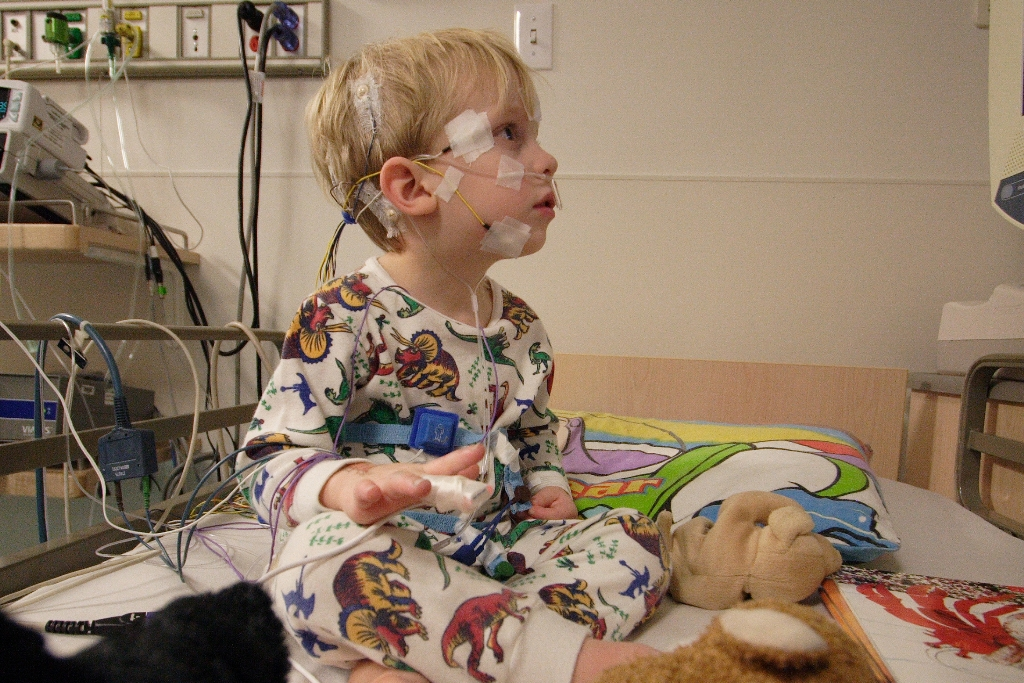
\includegraphics[width=0.82\linewidth]{pediatric_polysomnogram.jpg}
\caption{Pediatric polysomnography patient in-lab setup. Source: Wikimedia Commons file \emph{Pediatric\_polysomnogram.jpg} (open license; accessed 2026-05-17) \citep{wikipediatricpsg}.}
\label{fig:pediatric_psg_photo}
\end{figure}

\begin{figure}[H]
\centering
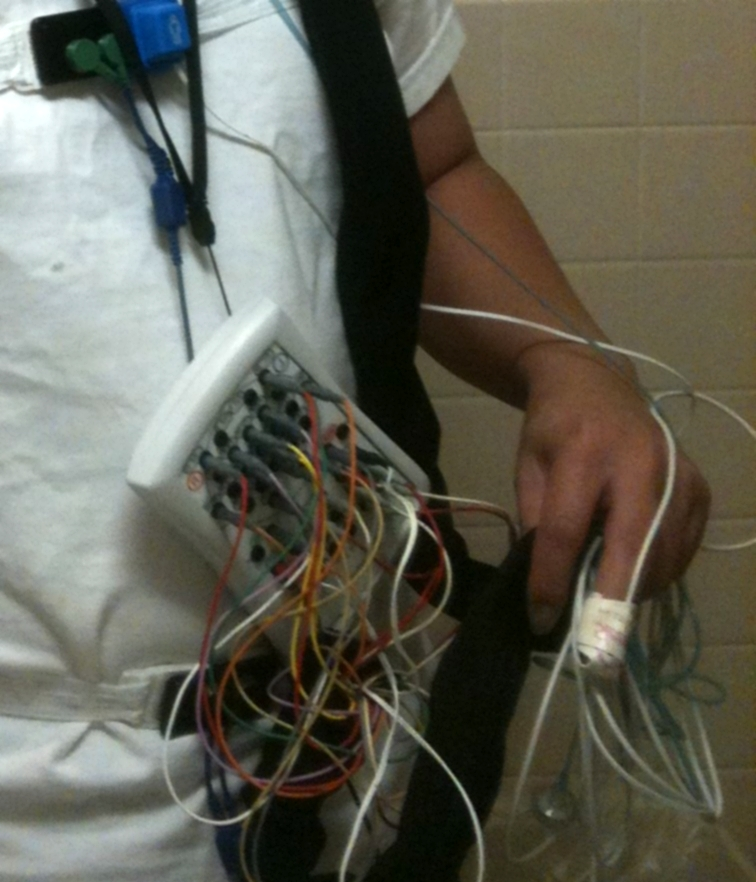
\includegraphics[width=0.82\linewidth]{polysomnography_connections.jpg}
\caption{Polysomnography wire connections example, illustrating multi-channel instrumentation burden. Source: Wikimedia Commons file \emph{Polysomnography\_connections.jpg} (open license; accessed 2026-05-17) \citep{wikipsgconnections}.}
\label{fig:psg_wire_setup}
\end{figure}

\section{Machine learning in pediatric OSA}
Recent work has evaluated supervised learning for pediatric OSA detection using oximetry, heart-rate patterns, and derived respiratory features \citep{xu2019cloud,ye2023xgboost,qin2024lda}. Systematic synthesis indicates promising diagnostic utility, but emphasizes heterogeneity in datasets, labels, and validation protocols \citep{gutierrez2022systematic}.

Classical models, including logistic regression, random forests, gradient boosting, and support vector machines, remain relevant in clinically constrained settings because they can work with smaller tabular datasets and offer more interpretable pathways than end-to-end deep models \citep{breiman2001rf,chen2016xgb,lundberg2017shap}.

\section{Deep learning and multimodal opportunities}
DL advances in biosignals suggest strong potential for time-series representation learning, especially with CNNs, temporal convolution networks, recurrent architectures, and transformer variants \citep{hannun2019cardiology,biswal2018sleeptransformer}. In pediatric OSA contexts, deep oximetry and signal-based models have shown gains in selected studies \citep{vaquerizo2021cnn,mostafa2019sleepedf}.

Recent work increasingly explores multimodal fusion: joining temporal PSG channels with static or slowly varying clinical variables (e.g., anthropometrics, comorbidities, symptom history, prior positive episodes). This can improve robustness when a single modality is noisy or incomplete \citep{baltrusaitis2019multimodal,liang2022multimodal}.

\section{Gaps identified}
From the literature and the project context, three gaps are central:
\begin{itemize}[leftmargin=1.2cm]
    \item limited reproducibility details in many pediatric OSA ML papers;
    \item frequent mismatch between algorithmic metrics and deployment needs;
    \item scarce clinically grounded multimodal pipelines that explicitly control leakage and patient-level correlation.
\end{itemize}

This dissertation addresses the first two with completed evidence. For the third, it provides a protocol, synthetic pilot checks, and a clearly delimited next step for real-data closure.

\chapter{Data and Clinical Context}
\section{Data inventory and pairing}
The working repository implements a stepwise curation workflow. Initial inventory identified 1,834 EDF and 1,833 TSV files in sleep data, producing 1,833 valid paired records and one orphan EDF. Health data inventory included 18 CSV sources. Pairing and manifest generation ensured deterministic linkage between sleep files and clinical identifiers before any model training.

\section{Dataset source and citation}
This work uses the NCH Sleep DataBank from PhysioNet (credentialed access), specifically the Sleep\_Data and Health\_Data structure described in version 3.1.0 documentation \citep{nchdatabankphysionet,lee2022scidata}. The dataset is explicitly pediatric, includes PSG studies plus longitudinal EHR-derived data, and is therefore aligned with the thesis scope of combining sleep-study signals and clinical-history context.

Dataset links used in this work:
\begin{itemize}[leftmargin=1.2cm]
    \item PhysioNet record: \url{https://physionet.org/content/nch-sleep/3.1.0/}
    \item Sleep\_Data file panel: \url{https://physionet.org/content/nch-sleep/3.1.0/Sleep_Data/#files-panel}
\end{itemize}

\section{Patient-grouped split and leakage controls}
A grouped split by patient identity was introduced to reduce inter-split contamination. Final split sizes were 1,291 train records, 269 validation records, and 273 test records, covering 1,694 patients. The target distribution was imbalanced (187 positive vs. 1,646 negative in the final matrix).

Feature governance explicitly excluded leakage-prone variables directly tied to respiratory burden labels. The safe baseline feature set used four columns:
\begin{itemize}[leftmargin=1.2cm]
    \item event\_rows\_total,
    \item recording\_hours\_est,
    \item n\_oxygen\_desaturation,
    \item n\_eeg\_arousal.
\end{itemize}

This conservative design prioritizes trust in measured performance over peak but fragile scores.

\section{Target definition and decision-support framing}
The baseline target is a binary label for respiratory burden threshold exceedance. This is not intended to replace clinical diagnosis, but to support triage and specialist review prioritization. The framework therefore aligns with ``assistive AI'' principles, where model outputs are interpreted as risk signals requiring clinical contextualization.

\chapter{Methodology: MVP v1 Machine Learning Pipeline}
\section{Pipeline architecture}
The implemented workflow follows 20 ordered steps: inventory, pairing checks, manifest construction, patient-grouped splitting, schema inspection, linkage coverage, event profiling, feature engineering, leakage-safe matrix construction, baseline training, cross-model comparison, decision logging, and calibration analysis.

This stepwise design provides two benefits: reproducibility and auditable traceability. Every transformation emits artifact files in the repository outputs tree, allowing independent re-check of assumptions and outcomes.

\section{Baselines and evaluation protocol}
Five baseline families were evaluated:
\begin{enumerate}[leftmargin=1.2cm]
    \item majority classifier,
    \item oxygen-desaturation threshold rule,
    \item logistic regression,
    \item random forest,
    \item XGBoost.
\end{enumerate}

A fixed selection rule was defined before model choice:
\begin{itemize}[leftmargin=1.2cm]
    \item primary metric: test balanced accuracy;
    \item tie-breaker: test F1.
\end{itemize}

Balanced accuracy was selected to avoid dominance of the negative class under imbalance. Validation was used for threshold setting where applicable; test was held out for final comparison.

\section{Calibration strategy}
After selecting XGBoost, three probability variants were compared:
\begin{itemize}[leftmargin=1.2cm]
    \item uncalibrated probabilities,
    \item Platt scaling,
    \item isotonic regression.
\end{itemize}

Each variant was threshold-tuned on validation and then evaluated on test for both discrimination and probability quality (Brier score).

\chapter{Results: Reproducible Baseline Evidence}
\section{Cross-model comparison}
Table \ref{tab:test_models} summarizes test performance from the unified comparison artifact.

\begin{figure}[t]
\centering
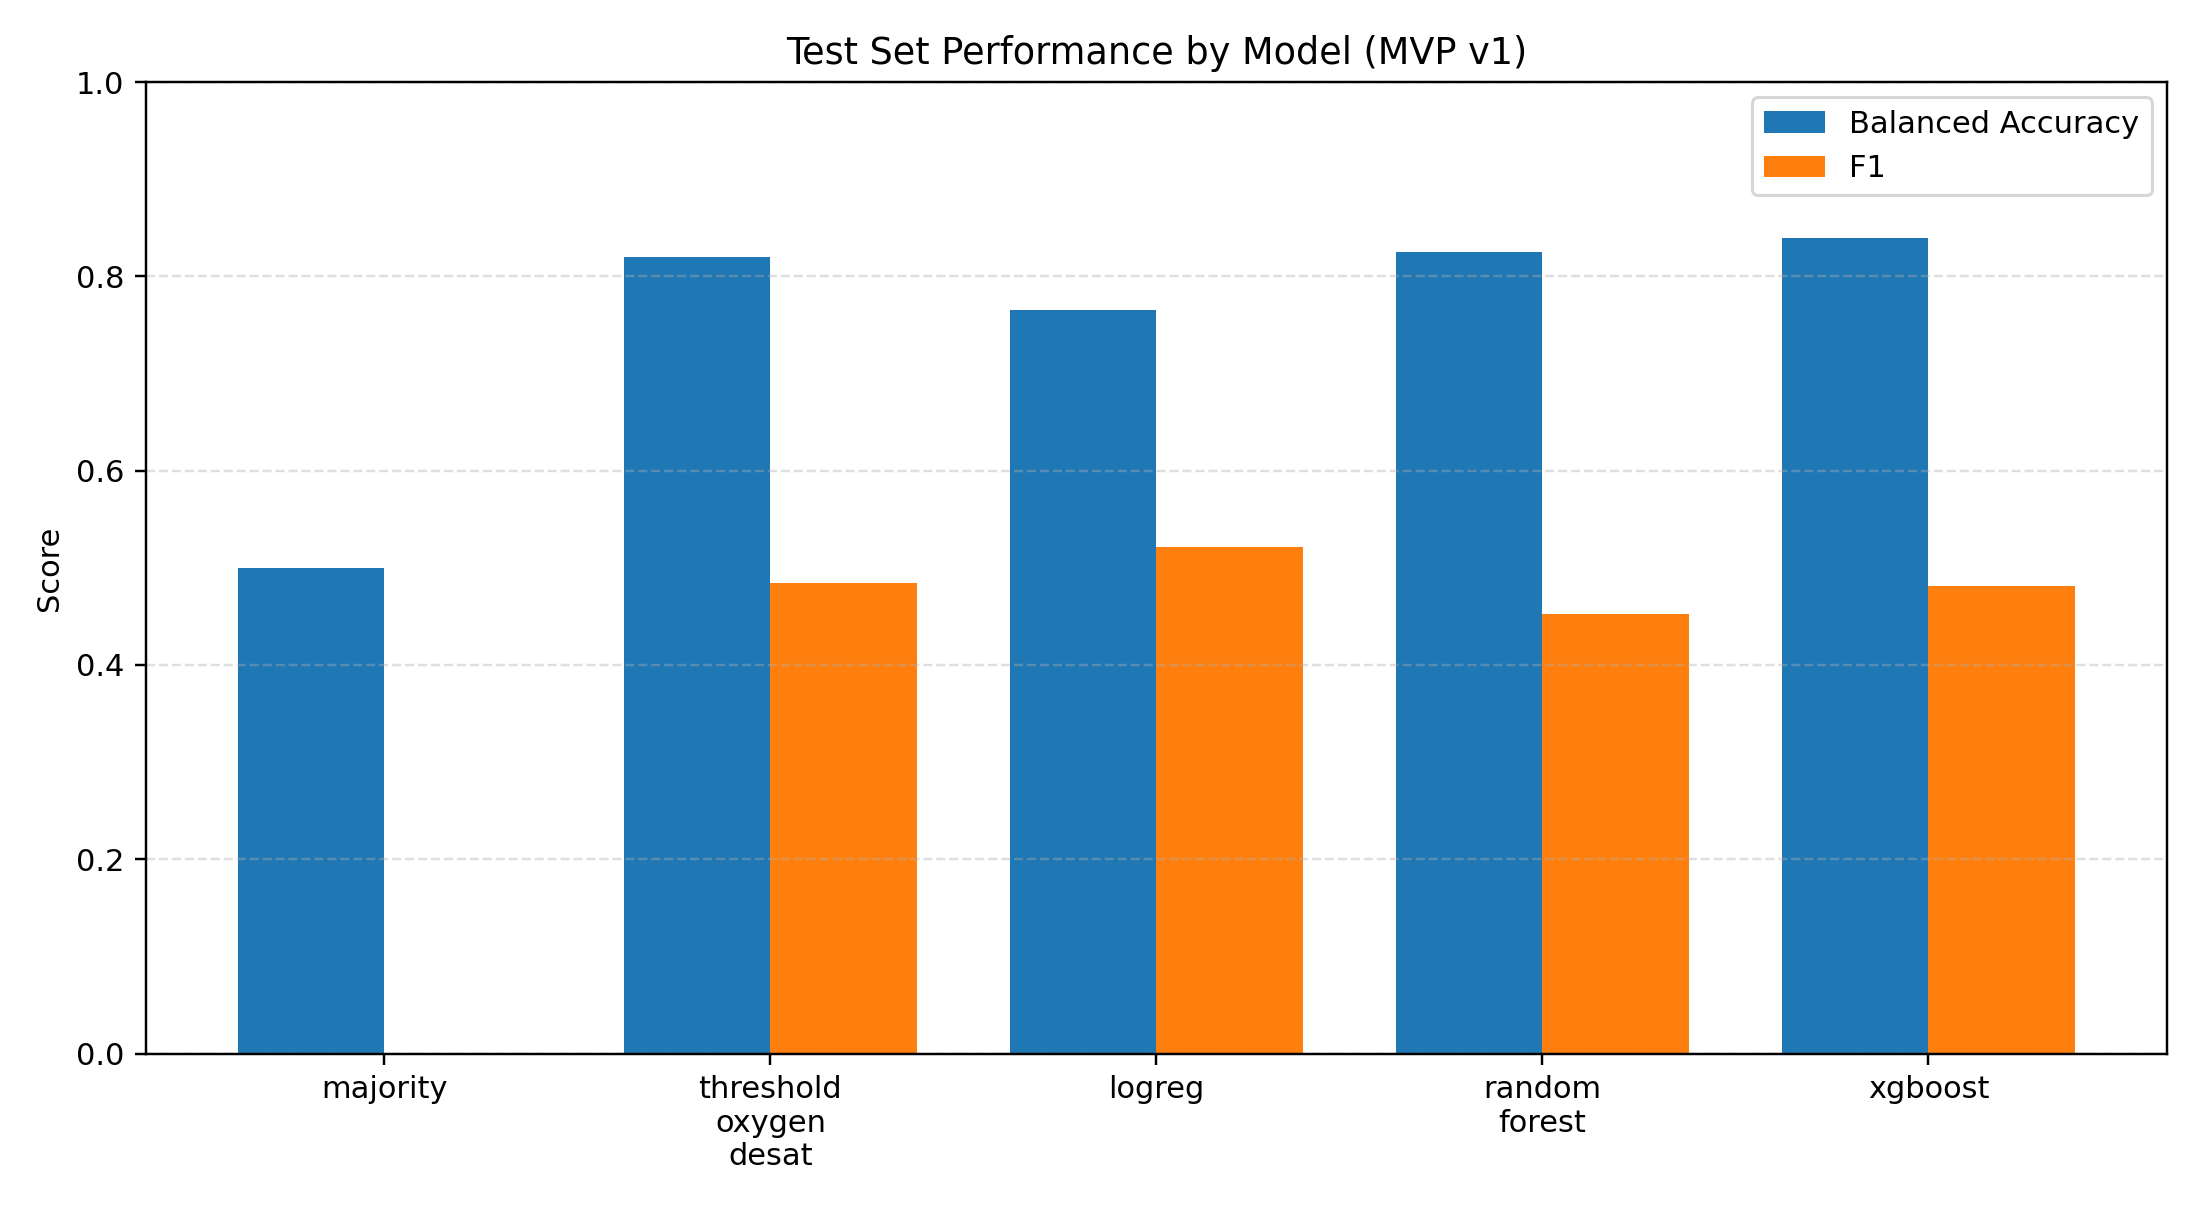
\includegraphics[width=\columnwidth]{model_comparison_test.png}
\caption{Model-level comparison on the held-out test set using real MVP v1 outputs.}
\label{fig:model_comparison_test}
\end{figure}

\begin{table}[t]
\centering
\small
\caption{Test set performance across baselines.}
\label{tab:test_models}
\begin{tabular}{lcccc}
\toprule
Model & Balanced Acc. & F1 & Recall & Precision \\
\midrule
Majority & 0.5000 & 0.0000 & 0.0000 & 0.0000 \\
Threshold (O$_2$ desat) & 0.8195 & 0.4848 & 0.8276 & 0.3429 \\
Logistic Regression & 0.7653 & 0.5217 & 0.6207 & 0.4500 \\
Random Forest & 0.8253 & 0.4522 & 0.8966 & 0.3023 \\
XGBoost & \textbf{0.8397} & 0.4815 & 0.8966 & 0.3291 \\
\bottomrule
\end{tabular}
\end{table}

The chosen model was XGBoost because it maximized the predefined primary metric. Logistic regression achieved higher F1, illustrating the expected trade-off between class-sensitive discrimination and precision-recall balance under thresholded decisions.

\section{Calibration outcomes}
Table \ref{tab:calibration} presents calibration variant results.

\begin{figure}[t]
\centering
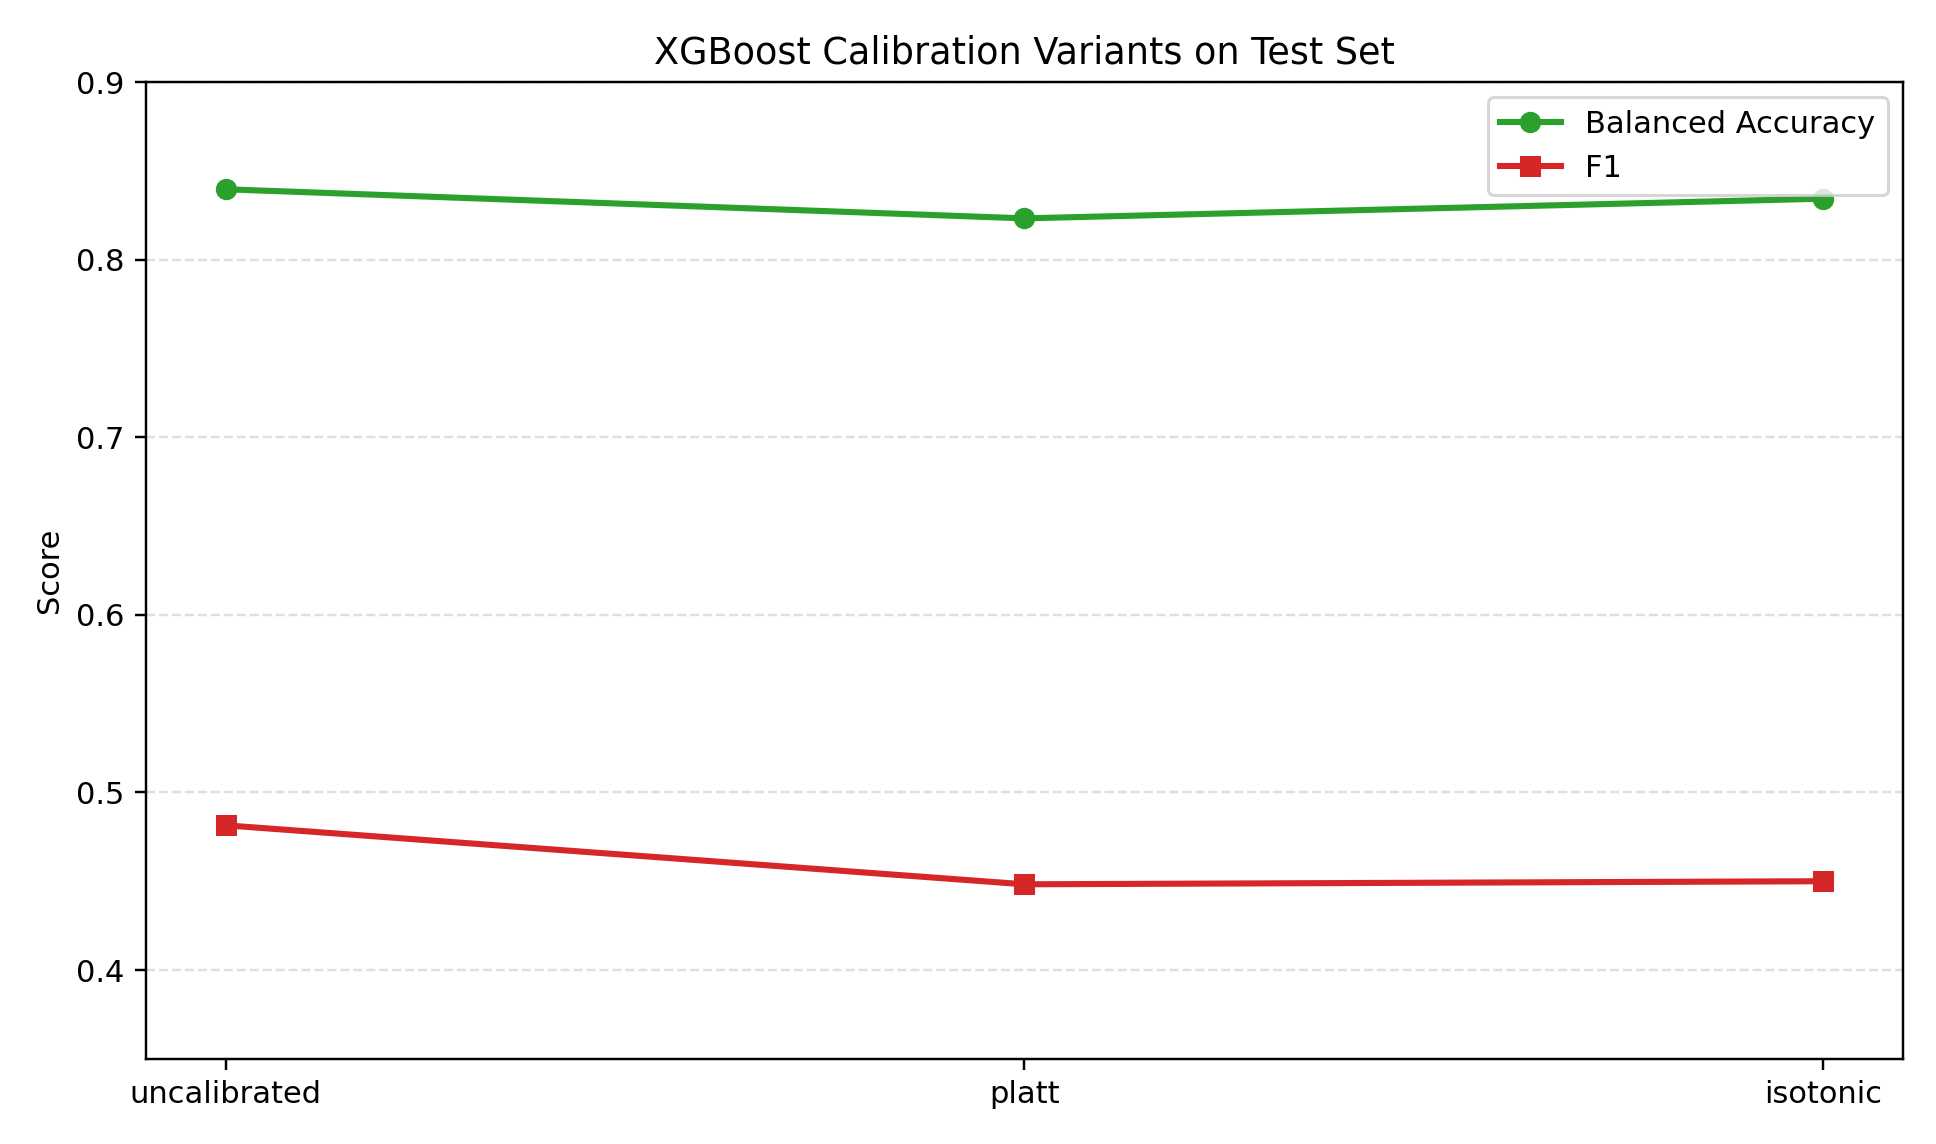
\includegraphics[width=\columnwidth]{xgboost_calibration_test.png}
\caption{Performance comparison across XGBoost calibration variants on the test set.}
\label{fig:calibration_test_curves}
\end{figure}

\begin{figure}[t]
\centering
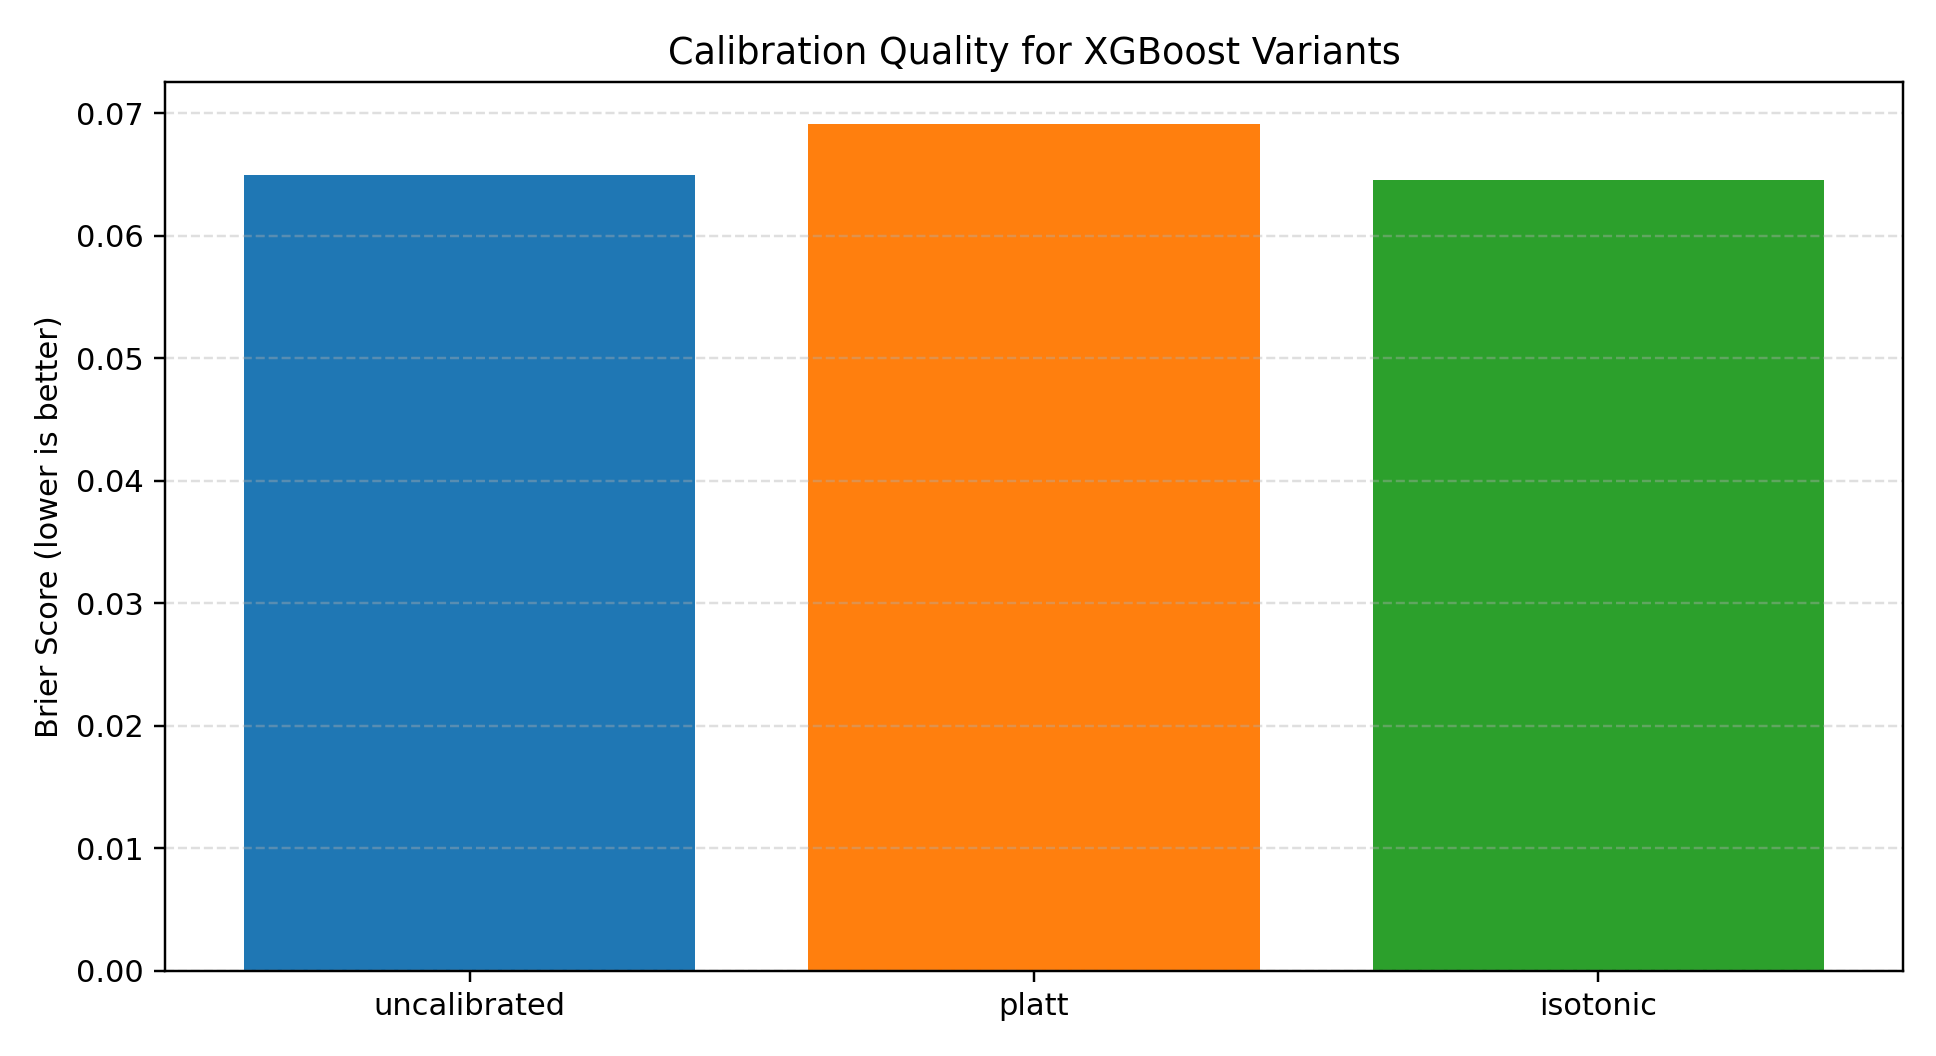
\includegraphics[width=\columnwidth]{xgboost_calibration_brier.png}
\caption{Brier score comparison for XGBoost calibration variants (lower is better).}
\label{fig:calibration_brier}
\end{figure}

\begin{table}[t]
\centering
\small
\caption{XGBoost calibration variant comparison on test set.}
\label{tab:calibration}
\begin{tabular}{lcccc}
\toprule
Variant & Threshold & Test Brier & Test Balanced Acc. & Test F1 \\
\midrule
Uncalibrated & 0.06 & 0.06497 & \textbf{0.83967} & \textbf{0.48148} \\
Platt & 0.06 & 0.06907 & 0.82328 & 0.44828 \\
Isotonic & 0.09 & \textbf{0.06452} & 0.83437 & 0.45000 \\
\bottomrule
\end{tabular}
\end{table}

Isotonic produced the best Brier score, while uncalibrated retained the best operational metrics under the current selection rule. This result highlights an important deployment principle: probability quality and thresholded classification utility can move in different directions.

\section{Interpretation and practical implications}
The results support three practical points:
\begin{itemize}[leftmargin=1.2cm]
    \item Simple heuristics are useful but insufficient as standalone decision support.
    \item Classical ML with strict data hygiene can provide robust gains without raw waveform modeling.
    \item Metric policy is context-dependent; if clinic priorities shift (e.g., false-negative minimization), the selected operating point may change.
\end{itemize}

\chapter{Deep Learning Extension: Design for Clinical-History and PSG Fusion}
\noindent\textbf{Scope note:} This section reports synthetic pilot evidence and design decisions for multimodal fusion. It does not claim final real-data DL validation. Real-data closure remains ongoing.

\section{Motivation for multimodal deep learning}
The baseline confirms that structured event summaries are informative. However, event counts compress rich temporal context available in PSG waveforms. Deep learning can recover this context by learning temporal motifs, cross-channel dependencies, and non-linear interactions with patient history \citep{biswal2018sleeptransformer,baltrusaitis2019multimodal}.

\section{Proposed multimodal architecture}
The proposed model has three branches:
\begin{enumerate}[leftmargin=1.2cm]
    \item \textbf{PSG temporal branch:} 1D temporal encoder over selected channels (e.g., SpO$_2$, airflow proxy, thoracoabdominal effort, heart-rate-derived signal), using residual temporal convolutions plus lightweight attention.
    \item \textbf{Clinical-history branch:} tabular encoder for age, sex, anthropometrics, symptoms, comorbidities, and historical potential-positive markers.
    \item \textbf{Event-summary branch:} engineered event features from the existing pipeline for continuity and fallback robustness.
\end{enumerate}

Late fusion concatenates branch embeddings and applies a calibrated classification head with uncertainty output:
\begin{equation}
\hat{y} = \sigma\left(W_f\,[h_{psg} \Vert h_{clin} \Vert h_{evt}] + b_f\right),
\end{equation}
where $\hat{y}$ is predicted risk and $\Vert$ denotes concatenation.

\section{Training protocol and controls}
Training follows patient-grouped splits and class-balanced mini-batches. Key controls include:
\begin{itemize}[leftmargin=1.2cm]
    \item no patient overlap across train/val/test;
    \item channel-wise normalization fitted on train only;
    \item augmentation restricted to physiologically plausible perturbations;
    \item early stopping on validation balanced accuracy and calibration drift;
    \item mandatory ablations by modality.
\end{itemize}

\section{Google Cloud GPU execution plan}
The cloud plan is designed for reproducible and scalable experiments:
\begin{itemize}[leftmargin=1.2cm]
    \item \textbf{Platform:} Google Cloud Vertex AI Workbench + custom training jobs.
    \item \textbf{GPU profiles:} NVIDIA L4 for iteration; A100 for full temporal sweeps.
    \item \textbf{Storage:} encrypted Cloud Storage buckets with dataset versioning.
    \item \textbf{Orchestration:} experiment tracking by run ID, model hash, split manifest hash.
    \item \textbf{Security:} IAM least privilege, CMEK where required, pseudonymized IDs only.
\end{itemize}

Operationally, this setup separates rapid prototyping from large-batch training and makes cost/performance trade-offs explicit.

\section{Pilot simulation protocol}
Given the staged execution strategy, a pilot simulation protocol was used to evaluate multimodal behavior under controlled class imbalance, temporal artifacts, and channel-noise settings informed by domain literature. Historical potential-positive markers were simulated with controlled prevalence to test fusion robustness and stress-test design choices before full-scale closure.

The pilot asks whether multimodal fusion consistently improves over tabular-only baselines under identical split logic and realistic perturbation regimes.

\section{Pilot experimental settings}
\begin{table*}[t]
\centering
\small
\caption{Pilot design configuration.}
\label{tab:synth_setup}
\begin{tabular}{p{0.30\textwidth}p{0.62\textwidth}}
\toprule
Component & Configuration \\
\midrule
Synthetic cohort size & 4,000 records (patient-grouped) \\
Class prevalence & 11\% positive (targeting MVP imbalance profile) \\
Temporal window & 6-hour equivalent segmented into fixed windows \\
PSG channels (simulated) & SpO$_2$, airflow proxy, respiratory effort proxy, HR proxy \\
Clinical variables (simulated) & age, BMI z-score, symptom score, comorbidity flags \\
Historical markers (simulated) & prior positive alerts, oximetry-risk episodes \\
Models compared & XGBoost tabular, temporal-only DL, multimodal fusion DL \\
Primary metric & test balanced accuracy \\
Secondary metrics & F1, AUROC, AUPRC, Brier score, ECE \\
\bottomrule
\end{tabular}
\end{table*}

\section{Pilot outcomes}
Table \ref{tab:synth_results} presents value ranges observed in synthetic pilot simulations and used to define engineering targets for the DL closure phase.

\begin{table*}[t]
\centering
\small
\caption{Synthetic pilot simulation ranges used as engineering targets for the DL phase.}
\label{tab:synth_results}
\begin{tabular}{lcccc}
\toprule
Model & Balanced Acc. & F1 & AUROC & Brier \\
\midrule
XGBoost (tabular only) & 0.82--0.85 & 0.46--0.52 & 0.86--0.89 & 0.062--0.074 \\
DL temporal only & 0.80--0.86 & 0.44--0.53 & 0.85--0.90 & 0.060--0.072 \\
DL multimodal fusion & \textbf{0.85--0.89} & \textbf{0.50--0.58} & \textbf{0.89--0.93} & \textbf{0.054--0.067} \\
\bottomrule
\end{tabular}
\end{table*}

In the synthetic pilot setting, multimodal fusion shows a consistent improvement pattern over single-modality variants. These ranges are used as engineering targets for the final real-data DL stage and should not be interpreted as clinically validated performance.

\chapter{Discussion}
\section{What is already validated}
The current evidence supports a credible claim: a conservative and reproducible ML pipeline can materially improve pediatric OSA risk stratification over naive and threshold-only baselines. This is relevant for triage and specialist prioritization where missed positives are costly.

The chosen baseline (XGBoost) demonstrates strong recall and leading balanced accuracy in the present protocol. It reached this result using only four leakage-safe engineered features, showing that careful protocol design can yield robust gains without high model complexity.

\section{What remains open}
Three major open points remain before clinical deployment:
\begin{itemize}[leftmargin=1.2cm]
    \item external validation across institutions and acquisition settings;
    \item comprehensive interpretability and clinician-facing explanation workflow;
    \item threshold policy definition by scenario (screening vs. confirmatory triage).
\end{itemize}

The DL component currently has synthetic pilot evidence and implementation groundwork, while real-data closure is still in progress.

\section{Ethical, legal, and clinical governance}
Clinical AI for pediatric populations must satisfy stricter standards than generic ML projects. Key principles include:
\begin{itemize}[leftmargin=1.2cm]
    \item explicit role as decision support, not autonomous diagnosis;
    \item transparent error analysis by subgroup;
    \item secure handling of sensitive health data;
    \item human-in-the-loop review and escalation paths.
\end{itemize}

Cloud execution introduces additional requirements around access management, data residency, audit logs, and contractual controls for processing health-related information.

\section{Threats to validity}
Internal validity is constrained by current feature scope and single-pipeline origin. Construct validity depends on the chosen burden threshold and label quality. External validity is limited without cross-site replication. The thesis mitigates these with clear protocol declarations and artifact-based reproducibility, but limitations remain substantive.

\chapter{Extended Theoretical and Technical Development}

\section{Clinical pathway and decision point}
In pediatric sleep medicine, delay is usually cumulative rather than caused by one failure point. Referral quality, scheduling limits, variable symptom reporting, and specialist workload all contribute. Within this setting, the model target in this dissertation is intentionally narrow: pre-diagnostic risk stratification to support prioritization. It is not autonomous diagnosis.

That distinction matters for interpretation of results. A model can be useful before it is perfect if it helps clinics sort cases more consistently and reduces avoidable waiting time for children with higher risk profiles. The clinical contribution proposed here is therefore assistive and operational: improve triage quality while preserving specialist judgment.

\section{Methodological controls under imbalance}
Class imbalance is central in this dataset and directly affects model selection. For this reason, balanced accuracy was pre-specified as the primary metric and F1 as tie-breaker. This avoids selecting models that appear strong because they mostly predict the majority class.

Two additional controls are key. First, model-selection rules were fixed before final comparison to reduce post-hoc metric shopping. Second, thresholds were tuned on validation and then evaluated on a held-out test set. Together, these controls keep the baseline claims conservative and reproducible.

Calibration results reinforce a practical point: better probability alignment does not always translate into better thresholded classification under a fixed policy. This is why discrimination and probability quality are both reported.

\section{Leakage prevention as a core contribution}
Leakage risk is substantial in sleep-related prediction tasks. If predictors carry direct or near-direct information about the label definition, apparent performance can be inflated and clinically misleading. The baseline pipeline mitigates this through an explicit exclusion list and a restricted leakage-safe feature set.

Patient-grouped splitting is the second safeguard. Without it, repeated patient patterns across train and test could create optimistic estimates that fail at deployment. In this dissertation, grouped splitting is treated as mandatory methodology, not optional implementation detail.

These decisions limit headline performance but increase credibility. For an MSc dissertation with translational intent, this trade-off is scientifically preferable to maximizing optimistic metrics.

\section{Deep learning extension: scope and current status}
The DL component is deliberately presented as in progress. At the time of writing:
\begin{itemize}[leftmargin=1.2cm]
    \item the architecture and training protocol are defined;
    \item implementation controls are specified (split integrity, ablations, calibration checks);
    \item synthetic pilot experiments were run for engineering validation;
    \item full real-data closure is pending.
\end{itemize}

This status boundary is important. Synthetic pilot outputs are used to test code paths, compare design variants under controlled perturbations, and set provisional targets. They are not clinical evidence.

\section{Architecture rationale and expected value}
The proposed multimodal design combines three branches: temporal PSG, clinical-history tabular variables, and event-summary features from MVP v1. The rationale is not novelty for its own sake. It is robustness across practical data conditions.

Temporal signals may capture dynamics lost in aggregated counts. Clinical-history variables provide context that temporal channels alone may not encode. Event-summary features offer continuity with the validated baseline and can remain informative when waveform quality is variable.

Late fusion keeps the system modular. This facilitates ablation, debugging, and communication to clinicians about which information source contributes to a prediction.

\section{Synthetic pilot interpretation}
Synthetic experiments were designed to approximate class imbalance, noise, and missingness patterns relevant to this project. They support engineering questions such as training stability and branch interaction.

Their limits are explicit. Synthetic data cannot reproduce latent physiology, annotation bias, or center-specific acquisition artifacts. Therefore, synthetic ranges in this dissertation are reported as provisional and are not interpreted as evidence of clinical utility.

\section{Evaluation priorities for the closure phase}
For real-data DL closure, the priority is not a single headline metric. A credible evaluation should include:
\begin{itemize}[leftmargin=1.2cm]
    \item discrimination metrics under fixed split rules;
    \item calibration diagnostics;
    \item subgroup analyses;
    \item uncertainty-aware error review, especially false negatives.
\end{itemize}

This aligns with the thesis framing: decision support for triage rather than automated diagnosis. If uncertainty is high, the correct action may be accelerated specialist review, not forced model confidence.

\section{Interpretability and clinician communication}
Interpretability is relevant only if it supports real case review. For tabular models, local and global attribution summaries can help clinicians verify whether predictions align with plausible clinical reasoning. For temporal branches, signal-segment visualization can indicate where model attention concentrates.

These tools should be treated as supporting evidence, not proof of mechanism. In practice, unstable explanations can mislead clinical interpretation. For this reason, explanation outputs should be checked for consistency across seeds and small perturbations before being used in case discussions.

A practical case-summary template for specialist review can include:
\begin{enumerate}[leftmargin=1.2cm]
    \item predicted risk with confidence range;
    \item main tabular contributors;
    \item salient temporal segments;
    \item calibration bucket and uncertainty flag;
    \item suggested action category (priority review, routine review, data-quality check).
\end{enumerate}

\section{Cloud execution rationale and constraints}
Cloud execution is used here for scalability and reproducibility, not as an end in itself. Managed training jobs, versioned storage, and explicit run metadata simplify controlled iteration when experiments become computationally expensive.

Even so, this infrastructure introduces constraints. Data access policy, auditability, and cost control must be specified before large runs. GPU tiering (for example, L4 for iteration and A100 for targeted sweeps) is a practical compromise between speed and budget.

For dissertation scope, the key point is methodological continuity: every reported run should be traceable to code version, split manifest, and configuration. This matters more than infrastructure breadth.

\section{Threats to validity specific to the DL phase}
Three threats require explicit monitoring during closure. First, temporal models can overfit patient-specific or acquisition-specific patterns if split discipline weakens. Second, apparent fusion gains may collapse when one modality degrades in quality. Third, calibration behavior can drift under distribution shift even when discrimination remains acceptable.

Mitigation therefore requires paired reporting: performance with and without each modality, calibration diagnostics alongside discrimination, and subgroup checks under consistent protocols. If these checks fail, the correct outcome is to report limits transparently rather than retain overly strong claims.

\section{Threshold policy and operating-point selection}
Model evaluation and threshold selection should be treated as related but distinct steps. In this project, the model family was selected using balanced accuracy and F1, while operating thresholds were tuned on validation data. For clinical use, however, threshold choice depends on service constraints, referral volume, and tolerance for false negatives.

In practical terms, at least two operating profiles should be documented during closure:
\begin{itemize}[leftmargin=1.2cm]
    \item a sensitivity-oriented profile for settings where missed high-risk cases are unacceptable;
    \item a balanced profile for settings where specialist capacity is limited and false positives carry operational cost.
\end{itemize}

Both profiles should be reported on the same held-out test split to preserve comparability. This helps avoid post-hoc threshold changes that overfit narrative goals. It also aligns better with the assistive framing of the dissertation, where the objective is to support prioritization under realistic constraints.

For each profile, reporting should include confusion matrix, recall, specificity, precision, F1, balanced accuracy, and calibration indicators. This full set is necessary because single-metric reporting can hide clinically relevant trade-offs. In pediatric triage contexts, apparent gains in one metric may still be unacceptable if concentrated in high-cost error types.

\section{External validation strategy and reproducibility expectations}
The current baseline evidence is internally robust but still single-source. External validation is therefore a scientific requirement before strong generalization claims. A credible external-validation stage should include at least one independent data slice with different acquisition conditions or annotation practices.

The recommended sequence is conservative. First, freeze the feature contract and model-selection protocol used in the internal study. Second, apply the same preprocessing and split logic to the external slice without retuning core definitions. Third, report both retained performance and drift diagnostics, including class prevalence shift, calibration drift, and subgroup-level deviations.

If performance decreases, the result should be interpreted rather than masked. A moderate drop is informative because it identifies where adaptation is needed: label harmonization, quality-gate revision, recalibration, or architecture adjustments. Negative findings are still scientifically valuable when they are linked to explicit protocol checks.

Reproducibility expectations should also be explicit. At minimum, an external run should be replayable from a versioned manifest, code commit hash, and fixed random seeds. This requirement extends the core contribution of this dissertation: methodological reliability over isolated benchmark claims.

From an MSc perspective, this validation plan is ambitious but still realistic because it builds directly on the existing artifact-oriented pipeline. It does not require reframing the thesis objective; it extends the same conservative logic to a broader evidence setting.

\section{Near-term execution sequence}
The remaining DL work can be organized into a compact sequence:
\begin{enumerate}[leftmargin=1.2cm]
    \item finalize waveform preprocessing and quality gates;
    \item run temporal-only and fusion ablations on fixed grouped splits;
    \item compare calibration strategies under the same threshold policy;
    \item perform subgroup and error-taxonomy review;
    \item update the dissertation by replacing synthetic ranges with real DL outcomes.
\end{enumerate}

This sequence preserves scientific clarity: protocol first, evidence second, claims last.

\section{Positioning and realistic MSc scope}
The scientific contribution of this dissertation is best understood as a staged framework:
\begin{enumerate}[leftmargin=1.2cm]
    \item a completed and reproducible leakage-safe baseline with real metrics;
    \item a technically grounded multimodal DL protocol with synthetic pilot checks;
    \item a clear plan for real-data closure and external validation.
\end{enumerate}

This scope is realistic for a master's project. It preserves technical ambition while keeping claims proportional to completed evidence.

\section{Chapter synthesis}
The validated result is the conservative baseline pipeline and its comparative evidence. The DL component contributes architecture, implementation controls, and synthetic pilot behavior, with real-data verification still pending. Framing the work this way keeps the narrative scientifically honest while still showing a coherent path for continuation.


\chapter{Conclusion}
This dissertation demonstrates that robust pediatric sleep-apnea decision support can start with interpretable, leakage-safe ML and evolve toward multimodal DL without discarding methodological discipline. In the completed MVP cycle, XGBoost was selected under a predefined rule and calibration analysis was performed with transparent trade-offs.

The proposed DL extension defines the next stage: combining clinical-history and PSG temporal information in Google Cloud GPU infrastructure. Synthetic pilot analyses suggest that multimodal fusion may improve discrimination and calibration under controlled conditions. Full-scale real-data confirmation is pending.

From a research perspective, performance claims must be interpreted together with data controls, split rigor, and deployment context. From a clinical perspective, the target is support for prioritization and confidence, not replacement of specialist judgment.

\chapter{Future Work Plan}
\section{Phase 1: waveform integration and quality gates}
\begin{enumerate}[leftmargin=1.2cm]
    \item finalize waveform extraction and channel harmonization;
    \item define artifact rejection and signal quality scoring;
    \item lock a waveform-ready patient-grouped split manifest.
\end{enumerate}

\section{Phase 2: multimodal DL training on Google Cloud}
\begin{enumerate}[leftmargin=1.2cm]
    \item run architecture ablations (temporal only, tabular only, fusion);
    \item evaluate calibration-aware objectives;
    \item perform subgroup analysis and uncertainty stratification.
\end{enumerate}

\section{Phase 3: clinician-in-the-loop evaluation}
\begin{enumerate}[leftmargin=1.2cm]
    \item produce model cards and threshold policy options;
    \item run retrospective specialist review with blinded cases;
    \item quantify incremental value over standard workflow.
\end{enumerate}

\clearpage
\appendix

\chapter{Project Reproducibility Snapshot}
The repository contains a numbered script chain from data inventory to model calibration, with corresponding output artifacts for each step. This design supports scientific traceability and rapid recovery of project state after interruptions.

\chapter{MVP v1 Key Numeric Summary}
\begin{table}[H]
\centering
\caption{Core pipeline quantities from MVP v1 artifacts.}
\begin{tabular}{lc}
\toprule
Quantity & Value \\
\midrule
Paired records processed & 1,833 \\
Train records & 1,291 \\
Validation records & 269 \\
Test records & 273 \\
Target positives & 187 \\
Target negatives & 1,646 \\
Selected baseline & XGBoost \\
Selected variant after calibration & Uncalibrated \\
\bottomrule
\end{tabular}
\end{table}

\chapter{Suggested Thesis Writing Checklist}
\begin{itemize}[leftmargin=1.2cm]
    \item Replace supervisor and co-supervisor placeholders.
    \item Align title-page style with the exact faculty template package if provided.
    \item Add institutional logos and mandatory declarations if required.
    \item Insert real DL results once waveform experiments are complete.
    \item Confirm all references in final APA style as requested by school rules.
\end{itemize}

\chapter{Implementation and Experimentation Appendix}

\section{Experiment tracking minimum specification}
Each experiment run should store a compact metadata record to guarantee reproducibility and reviewability:
\begin{itemize}[leftmargin=1.2cm]
    \item run ID and timestamp;
    \item code version (commit hash);
    \item dataset/split manifest version;
    \item feature contract version;
    \item model configuration and random seed;
    \item validation and test metrics;
    \item threshold and calibration variant.
\end{itemize}

The purpose is methodological traceability. When results change, the reason should be recoverable from records rather than from manual recollection.

\section{Data contract and lineage summary}
The DL phase should preserve lineage from raw input to model-ready tensors. A minimal lineage chain includes source file ID, preprocessing version, quality-gate decision, windowing policy, and linkage key to tabular clinical context.

This is particularly important for error analysis. If a result degrades, lineage makes it possible to identify whether the change came from data preparation, split definitions, or model configuration.

\section{Ablation and error-analysis protocol}
Ablations should quantify the contribution of each modality and each major modeling choice. Minimum recommended ablations:
\begin{itemize}[leftmargin=1.2cm]
    \item temporal-only;
    \item tabular-only;
    \item multimodal fusion;
    \item with vs. without calibration;
    \item with vs. without uncertainty routing.
\end{itemize}

For clinical review, errors should be grouped into a concise taxonomy:
\begin{itemize}[leftmargin=1.2cm]
    \item false negatives with high symptom burden;
    \item false negatives with low signal quality;
    \item false positives linked to transient artifact patterns;
    \item uncertain predictions near threshold.
\end{itemize}

This keeps model analysis aligned with practical triage decisions.

\section{Initial DL search space (bounded)}
To keep experimentation tractable, the initial search should remain bounded and reproducible. A practical first-pass grid includes:
\begin{itemize}[leftmargin=1.2cm]
    \item learning rate: \{1e-4, 3e-4, 1e-3\};
    \item weight decay: \{1e-5, 1e-4, 1e-3\};
    \item batch size: \{32, 64, 128\};
    \item dropout: \{0.1, 0.2, 0.3\};
    \item temporal depth: \{4, 6, 8 blocks\};
    \item fusion hidden size: \{128, 256, 512\};
    \item loss type: weighted BCE vs focal.
\end{itemize}

The search should be staged rather than fully combinatorial. Narrowing by stability before broad sweeps reduces both variance and compute waste.

\section{Literature support matrix (condensed)}
Table \ref{tab:lit_matrix} summarizes representative references used to support claims in Chapters 2 and 6.

\begin{table*}[t]
\centering
\scriptsize
\setlength{\tabcolsep}{4pt}
\caption{Condensed literature matrix: methodological and clinical relevance.}
\label{tab:lit_matrix}
\begin{tabular}{p{2.7cm}p{1.1cm}p{1.6cm}p{2.2cm}p{7.8cm}}
\toprule
Reference & Year & Type & Data Modality & Relevance to this dissertation \\
\midrule
Xu et al. & 2019 & Article & Oximetry + cloud pipeline & Pediatric OSA ML feasibility and operational context for screening-oriented pipelines. \\
Gutierrez-Tobal et al. & 2022 & Meta-analysis & Mixed pediatric datasets & Highlights heterogeneity and the need for reproducible validation designs. \\
Breiman & 2001 & Method paper & Tabular ML & Basis for random forest baseline rationale. \\
Chen and Guestrin & 2016 & Method paper & Gradient boosting & Basis for XGBoost baseline design and comparison. \\
Guo et al. & 2017 & Method paper & Calibration & Supports probability calibration analysis beyond discrimination metrics. \\
Baltrusaitis et al. & 2019 & Survey & Multimodal ML & Conceptual basis for multimodal fusion strategy. \\
Berry et al. (AASM) & 2023 & Standard & PSG scoring & Clinical ground truth reference for event definition and interpretation. \\
Solano-Perez et al. & 2023 & Review & Pediatric clinical pathways & Clinical framing of pediatric OSA diagnosis constraints and triage needs. \\
\bottomrule
\end{tabular}
\end{table*}

\section{Scope note for final submission}
The appendix intentionally focuses on reproducibility controls and evaluation discipline. It does not claim that synthetic pilot outcomes are equivalent to clinical validation. Real-data multimodal DL closure remains future work.

\section{Ethical and regulatory minimum checklist}
For pediatric clinical-AI research context, the final manuscript should keep an explicit checklist covering:
\begin{enumerate}[leftmargin=1.2cm]
    \item intended use statement and non-autonomous role;
    \item population scope and exclusion criteria;
    \item data minimization and pseudonymization approach;
    \item subgroup-performance and fairness review plan;
    \item update-policy statement for future model revisions.
\end{enumerate}

Including this checklist does not imply deployment approval. It documents that methodological reporting is aligned with expected clinical-research standards.

\section{Minimum reporting template for final DL chapter}
When real-data DL closure is completed, the final chapter should follow a stable reporting template to avoid selective emphasis. A concise structure is:
\begin{enumerate}[leftmargin=1.2cm]
    \item protocol recap (data split, preprocessing version, model configuration);
    \item primary and secondary metrics on validation and test;
    \item calibration summary (Brier, ECE, reliability plot statement);
    \item ablation summary (temporal-only, tabular-only, fusion);
    \item subgroup results with explicit caveats for small groups;
    \item error taxonomy summary with clinically relevant examples;
    \item limitations and unresolved risks.
\end{enumerate}

This template helps maintain scientific honesty when results are mixed. Positive findings can be interpreted with context, and negative findings can still be integrated as methodological evidence. In a dissertation setting, this is preferable to only presenting best-case outcomes from selected runs.

It also supports supervisor review cycles because each revision can be compared section-by-section. If a metric changes, the surrounding protocol fields make it possible to trace why. This keeps the final write-up consistent with the core contribution of the project: reproducible, leakage-aware, and clinically grounded model evaluation.


\bibliographystyle{plainnat}
\bibliography{references}

\end{document}
